\documentclass[11pt]{article}

%% ---------- packages ----------
\usepackage[margin=1in]{geometry}
\usepackage{amsmath, amssymb, amsthm}
\usepackage{graphicx}
\usepackage{hyperref}
\usepackage{booktabs}
\usepackage{float}
\usepackage{array}
\usepackage{enumitem}
\usepackage{natbib}          % author-year citations; swap for \usepackage{cite} if you prefer numbered
\usepackage{microtype}       % better text justification
\usepackage{xcolor}
\usepackage{caption}
\usepackage{subcaption}

%% ---------- custom commands ----------
\newcommand{\R}{\mathbb{R}}
\newcommand{\Rel}{\mathcal{R}}
\newcommand{\N}{\mathcal{N}}
\newcommand{\V}{\mathcal{V}}
\newcommand{\Y}{\mathcal{Y}}
\newcommand{\E}{\mathcal{E}}
\newcommand{\G}{\mathcal{G}}
\newcommand{\norm}[1]{\left\lVert #1 \right\rVert}

%% theorem-like environments
\newtheorem{theorem}{Theorem}[section]
\newtheorem{proposition}[theorem]{Proposition}
\newtheorem{lemma}[theorem]{Lemma}
\theoremstyle{definition}
\newtheorem{definition}[theorem]{Definition}
\newtheorem{remark}[theorem]{Remark}

%% ---------- metadata ----------
\title{\textbf{Graph Representation Learning,
       Relational GCNs, and Knowledge Graph Inference}}

\author{
  Adam Abramowitz \and
  Max Desantis \and
  Isaac Dreeben \and
  Abhi Mummaneni
}

\date{}   % leave blank or insert submission date

% ============================================================
\begin{document}

\maketitle
\thispagestyle{empty}

% ============================================================
\begin{abstract}

Much of modern data is relational — social networks, knowledge graphs, molecular structures, and narrative scenes all encode meaning through connections, not just attributes. This paper surveys the landscape of graph representation learning, tracing the development from classical spectral methods through graph convolutional networks, relational GCNs, and generative graph models. We then ground these ideas in two experiments using the Relational Graph Convolutional Network (R-GCN). First, we validate the architecture on a Wikidata temporal knowledge graph, demonstrating that relational message passing improves link prediction over a shallow baseline across all metrics. Second, we construct a novel dataset of over 500 murder mystery plots, using an LLM to extract relational knowledge graphs, and train the R-GCN to identify villains from circumstantial evidence alone. The model achieves 90.4\% accuracy and 0.762 villain $F_1$, with a $+14$-point precision advantage over a feature-only logistic regression baseline — a gap attributable specifically to typed relational structure rather than graph topology. The model further generalizes to a real unsolved case, producing suspect rankings consistent with current forensic evidence. Together, these results demonstrate that capturing typed relational structure leads to more effective learning across a diverse range of graph-structured problems.

\end{abstract}

\newpage
\tableofcontents
\newpage

% ============================================================
\section{Introduction}
\label{sec:intro}

Many real-world problems involve modeling highly structured graph data: social networks, knowledge graphs, time-series data, molecular structure, and much more. The challenge is to build models that capture deep structures beyond just surface level connections. We explore this challenge through both theory and practice. This paper will be divided into two parts. 

First we'll provide an expository survey of the modern techniques and models for embedding highly structured graphs for downstream tasks like deep learning and reconstruction. We'll trace the development of graph convolutional networks starting with the spectral methods we saw in class. We'll then see how these methods can be transformed into deeper generative models with richer latent spaces.

The second part of the paper will be a deep dive into modeling relational graphs via the Relation Graph Convolutional Network introduced by  Schlichtkrull et al. ADD CITATION HERE. We provide two experiments, both embedding relational graphs with the R-GCN architecture. The first graph is a Wikidata knowledge graph which we embed to demonstrate the effectiveness of embedding relational structure in addition to purely topological structure. Next, we use an LLM to generate knolwedge graphs of over $500$ detective story plots. We then embed these graphs with the R-GCN with the goal of predicting villains of the murder mysteries. The model then generalizes to predict the real-world Zodiac killer suspect. These experiments will show that capturing deeper structure leads to more effective learning across a diverse class of data types and settings. 




% ============================================================
\section{Structured Graph Representation Learning}
\label{sec:background}

% ----------------------------------------
\subsection{From Spectral Methods to Graph Convolutional Networks}
\label{subsec:spectral}

\subsubsection{Early Methods in Graph Learning}
Early graph-learning methods were motivated by the observation that graph structure can be used as an inductive bias for representation learning. In Laplacian Eigenmaps, Belkin and Niyogi \cite{belkin2001laplacian} construct a weighted graph over data points and seek low-dimensional embeddings that keep neighboring nodes close. Let $W$ be the weighted adjacency matrix, $D$ the diagonal degree matrix, and $L = D - W$ the combinatorial graph Laplacian. The embedding matrix $Y \in \mathbb{R}^{|V| \times d}$ is obtained by solving
\[
    \min_Y \; \frac{1}{2}\sum_{i,j} W_{ij}\|Y_i - Y_j\|_2^2
    = \min_Y \; \operatorname{tr}(Y^\top L Y),
    \qquad
    \text{s.t. } Y^\top D Y = I, \; Y^\top D\mathbf{1}=0.
\]
This objective makes the geometric assumption explicit: if two examples are adjacent in the graph, their learned representations should vary smoothly across that edge. The solution is given by the generalized eigenvectors of $L y = \lambda D y$, connecting graph embeddings to spectral approximations of the Laplace--Beltrami operator on an underlying manifold.

This smoothness viewpoint was further developed in manifold regularization \cite{belkin2006manifold}, where the graph is used to regularize functions defined on data points. For a graph signal $f : V \to \mathbb{R}$, the graph smoothness penalty is
\[
    \mathcal{R}_{G}(f)
    = \frac{1}{2}\sum_{i,j} W_{ij}\big(f_i - f_j\big)^2
    = f^\top L f.
\]
Thus, learning on graphs can be interpreted as learning functions whose values change slowly across high-weight edges. Shuman et al. \cite{shuman2013emerging} generalized this interpretation through the language of graph signal processing. If $L = U\Lambda U^\top$ is an eigendecomposition of the graph Laplacian, then the graph Fourier transform of a signal $x \in \mathbb{R}^{|V|}$ is
\[
    \widehat{x} = U^\top x,
    \qquad
    x = U\widehat{x}.
\]
Eigenvectors associated with small eigenvalues correspond to smooth, low-frequency variation over the graph, while larger eigenvalues correspond to high-frequency oscillations. This spectral viewpoint provides the foundation for defining graph convolutional filters.

\subsubsection{Graph Convolutional Networks}
Spectral graph neural networks extend convolution from Euclidean domains to irregular graph domains by filtering graph signals in the Laplacian eigenbasis \cite{bruna2014spectral,defferrard2016convolutional,kipf2017semi}. Given a signal $x$ and a spectral filter $g_\theta$, convolution can be written as
\[
    g_\theta * x
    = U g_\theta(\Lambda) U^\top x,
\]
where $g_\theta(\Lambda)$ scales each graph-frequency component independently. This formulation is expressive but depends on the eigendecomposition of the graph Laplacian, which is expensive for large graphs and not naturally transferable across graphs with different eigenbases.

Chebyshev spectral networks address this limitation by approximating the filter as a polynomial of the rescaled Laplacian \cite{defferrard2016convolutional}:
\[
    g_\theta * x
    \approx \sum_{k=0}^{K} \theta_k T_k(\widetilde{L})x,
    \qquad
    \widetilde{L} = \frac{2}{\lambda_{\max}}L - I,
\]
where $T_k$ denotes the $k$-th Chebyshev polynomial. Because this filter is a $K$-th order polynomial in $L$, it is localized to $K$-hop neighborhoods and avoids explicit eigendecomposition.

Kipf and Welling \cite{kipf2017semi} further simplified this construction by using a first-order approximation and a renormalized adjacency matrix. With self-loops $\widetilde{A}=A+I$ and degree matrix $\widetilde{D}_{ii}=\sum_j \widetilde{A}_{ij}$, a standard GCN layer is
\[
    H^{(\ell+1)}
    = \sigma\!\left(
        \widetilde{D}^{-1/2}\widetilde{A}\widetilde{D}^{-1/2}
        H^{(\ell)}W^{(\ell)}
      \right).
\]
This layer averages transformed node features over local neighborhoods, making GCNs an efficient and widely used architecture for semi-supervised node classification. However, repeated applications of the propagation operator can also cause node representations to become indistinguishable. Li, Han, and Wu \cite{li2018deeper} interpret GCN propagation as Laplacian smoothing; after $K$ propagation steps, the representation is dominated by powers of the normalized adjacency:
\[
    H^{(K)} \approx
    \left(\widetilde{D}^{-1/2}\widetilde{A}\widetilde{D}^{-1/2}\right)^K X.
\]
This smoothing perspective motivates later work on deeper GNNs, residual connections, attention mechanisms, and architectures designed to preserve long-range or high-frequency information.

\subsubsection{Graph Autoencoders and Generative Graph Models}
A second line of work relevant to graph representation learning comes from autoencoders and variational autoencoders. The variational autoencoder framework of Kingma and Welling \cite{kingma2014autoencoding} introduces a latent-variable model in which an encoder approximates the posterior distribution over latent variables and a decoder reconstructs the observed data. For data $x$, latent variable $z$, prior $p(z)$, encoder $q_\phi(z\mid x)$, and decoder $p_\theta(x\mid z)$, the evidence lower bound is
\[
    \mathcal{L}_{\mathrm{VAE}}(\theta,\phi;x)
    = \mathbb{E}_{q_\phi(z\mid x)}\big[\log p_\theta(x\mid z)\big]
      - \mathrm{KL}\!\left(q_\phi(z\mid x)\;\|\;p(z)\right).
\]
The first term encourages accurate reconstruction, while the KL term regularizes the latent space toward the prior. This framework naturally supports probabilistic generation by sampling from $p(z)$ and decoding.

Variational Graph Autoencoders (VGAEs) adapt this idea to graph-structured data by using a GCN encoder and an edge-probability decoder \cite{kipf2016variational}. Given node features $X$ and adjacency matrix $A$, the encoder factorizes over nodes as
\[
    q_\phi(Z\mid X,A)
    = \prod_{i=1}^{|V|} q_\phi(z_i\mid X,A),
    \qquad
    q_\phi(z_i\mid X,A)
    = \mathcal{N}\!\left(z_i\mid \mu_i,\operatorname{diag}(\sigma_i^2)\right),
\]
and the decoder predicts edges through an inner product:
\[
    p_\theta(A_{ij}=1\mid z_i,z_j)
    = \sigma(z_i^\top z_j).
\]
This model connects graph representation learning with link prediction: the latent embedding must encode enough structural information to reconstruct the observed adjacency matrix.

Subsequent generative graph models extend VGAEs from link prediction toward whole-graph generation. GraphVAE \cite{simonovsky2018graphvae} decodes latent variables into probabilistic node and edge tensors for small graphs, while Graphite \cite{grover2019graphite} improves the decoder by iteratively refining a generated graph. These models can be viewed as learning a distribution over graphs,
\[
    p_\theta(G)
    = \int p_\theta(G\mid z)p(z)\,dz,
\]
where the decoder must capture both local edge dependencies and global graph-level constraints. This generative perspective complements discriminative GNNs by emphasizing reconstruction, latent structure, and graph synthesis.

\subsubsection{Relational Graphs and Relational GCNs}
\label{subsec: rel_graphs}
Many real-world graphs are not homogeneous: edges may represent different relation types, and nodes may belong to different semantic categories. Relational GCNs extend the GCN update rule to multi-relational graphs by assigning relation-specific transformations \cite{schlichtkrull2018modeling}. For relation set $\mathcal{R}$, relation-specific neighborhood $\mathcal{N}_i^r$, and normalization constant $c_{i,r}$, the R-GCN update is
\[
    h_i^{(\ell+1)}
    = \sigma\!\left(
        \sum_{r\in\mathcal{R}}\sum_{j\in\mathcal{N}_i^r}
        \frac{1}{c_{i,r}} W_r^{(\ell)}h_j^{(\ell)}
        + W_0^{(\ell)}h_i^{(\ell)}
      \right).
\]
This formulation separates messages by relation type, making it suitable for knowledge graphs and other structured domains in which edge labels carry semantic meaning.

Heterogeneous graph models further generalize this idea by allowing both node-type-specific and edge-type-specific transformations. The Heterogeneous Graph Transformer of Hu et al. \cite{hu2020heterogeneous} uses attention mechanisms whose parameters depend on the source node type, target node type, and relation type. A simplified relation-aware attention score can be written as
\[
    \alpha_{ij}^{r}
    = \operatorname{softmax}_{j\in\mathcal{N}_i^r}
      \left(
      \frac{(Q_{\tau(i)}h_i)^\top R_r(K_{\tau(j)}h_j)}{\sqrt{d}}
      \right),
\]
where $\tau(i)$ denotes the type of node $i$ and $r$ denotes the relation connecting nodes $i$ and $j$. This line of work shows how similarity graphs used in early spectral methods can be extended to typed, relational, and semantically structured graphs.

\subsubsection{Message Passing, Attention, and Graph Transformers}
Message passing provides a unifying abstraction for many GNN architectures. Gilmer et al. \cite{gilmer2017neural} formulate neural message passing in terms of a message function, aggregation operation, and update function. At layer $t$, a generic message passing update is
\[
    m_i^{(t+1)}
    = \sum_{j\in\mathcal{N}(i)} M_t\!\left(h_i^{(t)}, h_j^{(t)}, e_{ij}\right),
    \qquad
    h_i^{(t+1)}
    = U_t\!\left(h_i^{(t)}, m_i^{(t+1)}\right).
\]
GCNs, R-GCNs, and many spectral approximations can be interpreted as instances of this template with different choices of message function, normalization, and aggregation.

Graph Attention Networks make the connection between message passing and attention explicit by replacing fixed neighborhood averaging with learned attention weights \cite{velickovic2018graph}. For neighboring nodes $i$ and $j$, attention coefficients are computed as
\[
    \alpha_{ij}
    = \operatorname{softmax}_{j\in\mathcal{N}(i)}
      \left(
      \operatorname{LeakyReLU}\!\left(a^\top[Wh_i\,\|\,Wh_j]\right)
      \right),
\]
and the node update becomes
\[
    h_i'
    = \sigma\!\left(\sum_{j\in\mathcal{N}(i)} \alpha_{ij}Wh_j\right).
\]
Attention allows the model to assign different weights to different neighbors, rather than assuming that all adjacent nodes contribute equally.

Transformer-style graph models generalize this principle by combining global or constrained attention with structural encodings. Dwivedi and Bresson \cite{dwivedi2020generalization} adapt Transformers to arbitrary graphs using graph-aware positional encodings, while Graphormer \cite{ying2021transformers} demonstrates that full attention can be effective when enriched with structural biases such as shortest-path distances and edge encodings. A common way to express graph-biased attention is
\[
    \operatorname{Attn}(Q,K,V;B)
    = \operatorname{softmax}\!\left(\frac{QK^\top}{\sqrt{d}} + B\right)V,
\]
where $B_{ij}$ encodes graph structure. In constrained attention, one may set
\[
    B_{ij}=
    \begin{cases}
    0, & (i,j)\in E \text{ or } i=j,\\
    -\infty, & \text{otherwise},
    \end{cases}
\]
which recovers neighborhood-restricted attention; richer choices of $B$ permit long-range interactions while preserving graph inductive bias. Recent graph language models \cite{plenz-frank-2024-graph} further connect this line of work to language modeling by incorporating graph structure into pretrained, Transformer-like architectures.

\subsubsection{Expressivity and Limitations}
Although message passing architectures are broadly useful, their expressivity is limited. 
Xu et al. \cite{xu2019powerful} relate the discriminative power of GNNs to the Weisfeiler--Lehman (WL) graph isomorphism test. 
In WL-style refinement, node colors are updated by hashing the previous color together with the multiset of neighboring colors:
\[
    c_i^{(k)}
    = \operatorname{HASH}\!\left(
        c_i^{(k-1)},
        \left\{c_j^{(k-1)} : j\in\mathcal{N}(i)\right\}
      \right).
\]
Similarly, standard message passing GNNs update node embeddings by aggregating multisets of neighbor representations. As a result, many GNNs cannot distinguish graph structures that the 1-WL test cannot distinguish.

A separate limitation is over-squashing: information from a large receptive field must be compressed into fixed-dimensional node embeddings. After $T$ message passing layers, a node representation can depend on all nodes within $T$ hops,
\[
    h_i^{(T)}
    = \Phi_T\!\left(\left\{x_j : \operatorname{dist}(i,j)\leq T\right\}\right)
    \in \mathbb{R}^d,
\]
but the dimension $d$ remains fixed even when the number of contributing nodes grows exponentially with distance. Alon and Yahav \cite{alon2021bottleneck} identify this bottleneck as a practical obstacle for long-range reasoning on graphs.

These limitations motivate architectures that augment message passing with virtual edges, positional encodings, higher-order structures, or global attention.
However, as seen in \cite{velickovic2022message} many approaches that appear to go beyond message passing can be reframed as message passing over an augmented graph,
\[
    G' = (V',E'),
    \qquad
    E \subseteq E',
\]
where added edges, nodes, or features change the computational graph over which information flows.
In conclusion, though the many GCN architectures and graph learning methods seem distinct, each can be understood in the context of the Laplacian of the graph and distinguiched by their choices of graph structure, message aggregation, and inductive bias.

% ----------------------------------------
\subsection{Deeper Autoencoders: VAEs and Adversarial Autoencoders}
\label{subsec:autoencoders}

\subsection{Generative Adversarial Networks}
Goodfellow et al. introduced Generative Adversarial Nets, which optimize two functions G and D through the following min-max objective:

\[
\min_G \max_D V(D,G)
=
\mathbb{E}_{x \sim p_{\text{data}}(x)}
\left[\log D(x)\right]
+
\mathbb{E}_{z \sim p_z(z)}
\left[\log\left(1 - D(G(z))\right)\right].
\]

D must discriminate between the prior data distribution \(p_{\text{data}}\), and the generator's output G(z), with \(z \sim p_z\). 

The resultant Nash equilibrium is that G learns to model \(p_{data}\), and D cannot distinguish between generated samples and samples from \(p_{data}\). Note that this only requires the ability to sample from the prior distribution. This enables a generalization of VAEs towards more complex and hard to define latent regularizations. It is also important to note that, as Goodfellow et. al mention, memorization is less likely in a GAN as information from the prior distribution does not flow directly into the generator.

\subsubsection{Adversarial Autoencoders}
Makhzani et al. connect GANs and autoencoders by using GANs to regularize the latent space. A traditional variational autoencoder looks to minimize the following:
\[
    \mathcal{L}_{\mathrm{VAE}}(\theta,\phi;x)
    = -\mathbb{E}_{q_\phi(z\mid x)}\big[\log p_\theta(x\mid z)\big]
      + \mathrm{KL}\!\left(q_\phi(z\mid x)\;\|\;p(z)\right).
\]

This however requires being able to form \[q_\theta(z\mid x)\] which is not a probability distribution in a deterministic encoder. Consider a standard autoencoder. How would you produce a distribution over latents for a given data point? Adversarial Autoencoders introduce the aggregated latent, which is a distribution over all of the latent variables, not just the latent distribution for a given data point.
\[
q(z) = \int_x q(z \mid x)\, p_d(x)\, dx
\]

Then the autoencoder is trained using alternating minimization, where first the autoencoder is trained to accurately reconstruct the inputs:
\[
L = \frac{1}{N}\sum_{i=1}^{n} (y_i-D(z_i))^2 \quad \text{with} \quad z_i = E(x_i)
\]
where E is the encoder, D is the decoder, $(x_i, y_i)$ is the labeled training data.
Afterwards, the model is trained to minimize:
\[
\min_E \max_H V(H,E)
=
\mathbb{E}_{x \sim p_{\text{data}}(x)}
\left[\log H(x)\right]
+
\mathbb{E}_{z \sim p_z(z)}
\left[\log\left(1 - H(E(z))\right)\right].
\]

where E is the encoder and H is the discriminator.


\subsubsection{Adversarially Regularized Graph Autoencoders}
Pan et al. combined concepts from VGAEs and AAEs to use adversarial methods to regularize the latent space of graph autoencoders. They use a Graph Convolutional Network for their encoding model, and 
\[
p\!\left(\hat{A}_{ij}=1 \mid z_i, z_j\right)
=
\sigma\!\left(z_i^\top z_j\right)
\]
as their decoder for link prediction.

The paper used two concepts from adversarial autoencoders: the aggregated latent and the alternating minimization scheme between minimization reconstruction loss and adversarially regularize the latent space. For reconstruction loss minimization, the authors propose using the log-likelihood
\[
L_0
=
\mathbb{E}_{q(Z \mid X,A)}
\left[
\log p(\hat{A}\mid Z)
\right]
\]

for deterministic models, but also propose using
\[
L_1
=
\mathbb{E}_{q(Z \mid X,A)}
\left[
\log p(\hat{A}\mid Z)
\right]
-
\mathrm{KL}
\left[
q(Z\mid X,A)
\,\|\, 
p(Z)
\right]
\]
for variational models, thus using both VAE regularization and adversarial regularization.

In both cases, Z are the latent vectors, A is the adjecency matrix, and X are node features.


% ============================================================
\section{Experiments: R-GCN Deep Dive}
\label{sec:experiments}

We now turn from our exposition on structured graph learning to two applications of the relational graph convolutional network (R-GCN) model introduced by Schlichtkrull et al. [?] ADD CITATION HERE. First, we embed a wikidata temporal knowledge graph with the goal of link prediction. We chose this dataset to demonstrate that the R-GCN message passing technique improves predictive capabilities over naive models that don't see the relational structure. Secondly, we test the R-GCN encoder on an entity classification task with a knowledge graph built from detective stories in movies, novels, TV shows, etc. 



% ============================================================
\subsection{Wikidata Knowledge Graph}
\label{subsec:wikidata}

Before applying the R-GCN to the detective corpus,
we first validate it on tkgl-smallpedia, a temporal knowledge
graph benchmark drawn from Wikidata~\citep{tgb2023} CITATION HERE.
The dataset consists of ordered quadruples $(s, r,o, t)$ encoding
that entity $s$ is related to entity $o$ by relation $r$ at time $t$. Entities are Wikidata items (persons, cities, institutions, awards, etc.,)
and relations are Wikidata properties (member of sports team, country of citizenship, award received, doctoral student, etc.). Table~\ref{tab:wiki_stats} provides some dataset statistics and Figure \ref{fig: smallpedia_subgraph} shows a subgraph of some of the nodes connected to the Kingdom of Italy for a visual example. 
\begin{figure}[H]
    \centering
    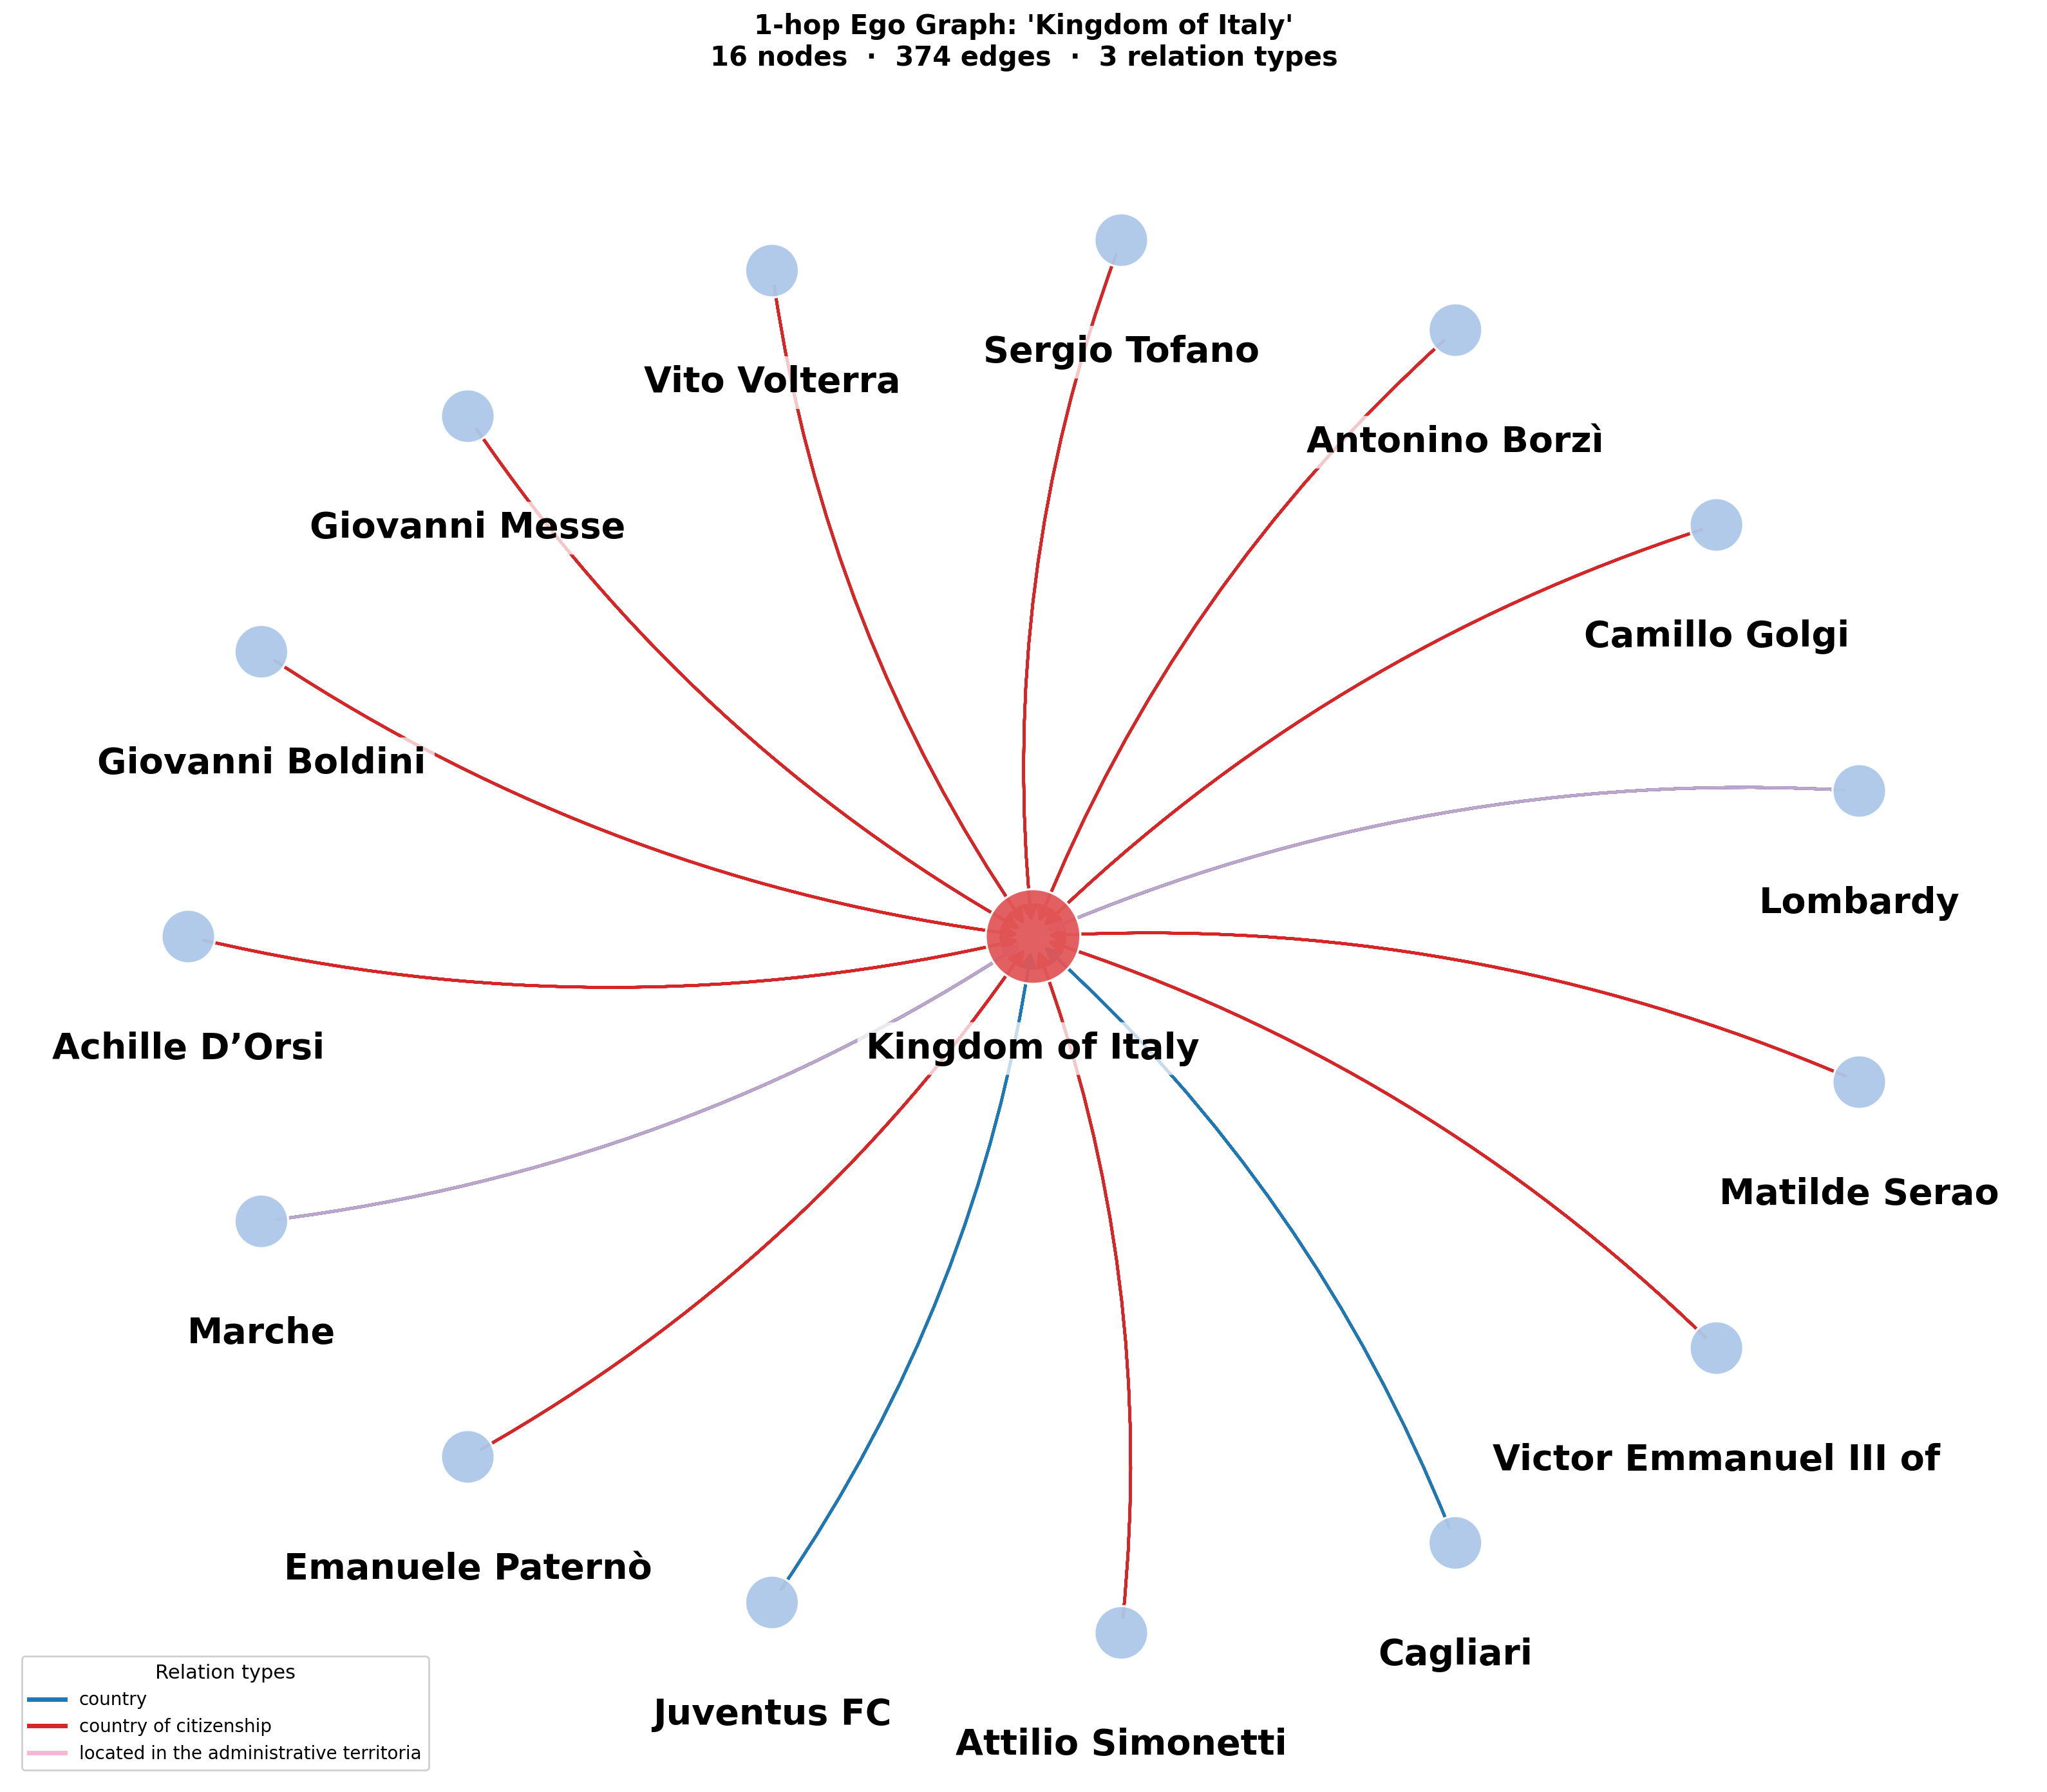
\includegraphics[width=0.5\linewidth]{fig3_ego_graph.png}
    \caption{Subgraph of the tkgl-smallpedia dataset. The red edges have the relation \emph{Country of Citizenship}, the blue edges have the relation \emph{Country}, and the purple edges have the relation \emph{located in the administrative territorial entity}.}
    \label{fig: smallpedia_subgraph}
\end{figure}For the purpose of this experiment, we will ignore the time dependence term $t$ for each edge and view our task as static link prediction: given any two entries of the triple, $(s,r,o)$, predict the third, among all entities (or relations). 

The purpose of this experiment is specifically to isolate the contribution
of relational message passing.  To that end, we compare two models that share an identical DistMult decoder~\citep{yang2015embedding} but differ in
how entity representations are produced:

\begin{itemize}
  \item \textbf{Shallow DistMult.}  Each entity receives a learned
    embedding with no graph encoder.  The decoder scores a triple
    with the scoring function $f(s,o,r) = h_s^\top R_rh_o$. This baseline captures co-occurrence statistics
    but ignores the graph structure entirely.


  \item \textbf{R-GCN + DistMult.}  First, we embed our feature matrix $X^0$ with a two-layer R-GCN encoder
    (hidden dimension 64, 30 basis matrices, dropout 0.1). Then train on the same DistMult scoring and loss function. 
\end{itemize}

Both models are trained for 50 epochs with the Adam optimiser
(learning rate $10^{-3}$, batch size 4{,}096) using binary
cross-entropy loss against one randomly corrupted negative per
positive triple.  Evaluation follows the filtered ranking protocol
with 50 negatives per positive on the held-out test split.
\begin{table}[H]
\centering
\begin{minipage}{0.45\linewidth}
\centering
\begin{tabular}{lr}
\toprule
Property & Value \\
\midrule
Temporal edges  & 1,100,752  \\
Unique nodes    & 47,433     \\
Relation types  & 566        \\
Time span       & 1900--2024 \\
\bottomrule
\end{tabular}
\end{minipage}
\hfill
\begin{minipage}{0.45\linewidth}
\centering
\begin{tabular}{lr}
\toprule
Split      & Edges   \\
\midrule
Training   & 775,514 \\
Validation & 162,066 \\
Test       & 163,172 \\
\bottomrule
\end{tabular}
\end{minipage}
\caption{Dataset statistics for tkgl-smallpedia.}
\label{tab:wiki_stats}
\end{table}
% ----------------------------------------
\subsubsection{Results}
\label{subsubsec:wikidata-results}

Table~\ref{tab:wikidata} reports Mean Reciprocal Rank (MRR) and
Hits@$K$ for $K \in \{1, 3, 10\}$ on the test set.

\begin{table}[H]
\centering
\begin{tabular}{lcccc}
\toprule
Model               & MRR    & Hits@1 & Hits@3 & Hits@10 \\
\midrule
Shallow DistMult    & 0.2238 & 0.1739 & 0.2084 & 0.2676 \\
R-GCN + DistMult    & \textbf{0.2900} & \textbf{0.2026} 
                    & \textbf{0.2690} & \textbf{0.4698} \\
                    
\bottomrule
\end{tabular}
\caption{Link prediction on \textsc{tkgl-smallpedia} (test set,
         50 negatives per positive, filtered ranking).
         Best result per metric in \textbf{bold}.}
\label{tab:wikidata}
\end{table}

The R-GCN encoder improves over the shallow baseline across all
four metrics, with relative gains of $+29.6\%$ in MRR,
$+16.5\%$ in Hits@1, $+29.1\%$ in Hits@3, and $+75.6\%$
in Hits@10.

\subsubsection{Discussion}
\label{subsubsec:wikidata-discussion}

State-of-the-art link prediction methods on knowledge graphs have Hits@$K$ hovering around 0.6. So, our R-GCN encoder is not quite there. However, we do see that the R-GCN encoder does strictly improve every metric across the board compared to the unstructured shallow DistMult baseline. The most striking result is the Hits@10 improvement: the R-GCN
places the correct object in the top 10 candidates for nearly
half of all test queries (0.4698), compared to only one quarter
for the shallow baseline (0.2676). Some Hits@1 and Hits@3 but large gains with Hits@10 is consistent with what one would expect from a structural encoder.  The R-GCN does not
always rank the single correct answer first, but it reliably
pulls it into the set of plausible candidates by recognizing that
entities sharing similar relational neighborhoods are likely to
participate in similar triples.  The shallow model, lacking any
notion of neighborhood, relies entirely on direct co-occurrence
statistics and so it struggles to generalize to less-frequent
entities or relation types.



The small, but still positive, MRR and Hits@1 gains ($+29.6\%$ and $+16.5\%$ respectively) may reflect the difficulty of
precise top-1 ranking on a knowledge graph with ambiguous entities.
The asymmetry between Hits@1 and Hits@10 suggests there is still
room for improvement in the encoder. For instance, we could implement tighter hyperparameter tuning, attention-weighted message passing
(cf.\ Graph Attention Networks~\citep{velickovic2018graph}), CITATION HERE
or we could have incorporated the temporal index $t$ that we set aside for this
experiment. One additonal shortfall of the DistMult scoring function $f(s,r,o) = h_s^\top R_r h_o$ is that it is bidirectional. The matrix $R_r$ is diagonal which means $h_s^\top$ and $h_o$ commute through $R_r$, i.e., $h_s^\top R_rh_o = h_o^\top R_r h_s$. So, the model scores ``$A$ is related to $B$" the same as ``$B$ is related to $A$." Adding synthetic triples $(o,r^{-1}, s)$ with reverse edges would solve this issue. We implement this change to address the obvious bidirectional issue with the murder mystery experiment. But, implementing this change for tkgl-smallpedia may also improve the DistMult scoring metrics.

Just to see how the scoring function operates, if we ask to predict the object in the incomplete triple (Marie Curie, Winner, ?), the top 5 predicted objects with their scores are shown in Table \ref{tab:curie}. 

\begin{table}[H]
\centering
\begin{tabular}{clr}
\toprule
Rank & Predicted Entity & Score \\
\midrule
1  & Nobel Prize in Chemistry$^\dagger$ & 5.0768 \\
2  & Eddington Medal                    & 4.3701 \\
3  & Nobel Prize in Physics$^\dagger$   & 3.5951 \\
4  & National Medal of Science          & 3.5567 \\
5  & Henry Draper Medal                 & 3.4259 \\
\bottomrule
\end{tabular}
\caption{Top-5 predicted completions for the query
         (Marie Curie, winner, ?). 
         Factually correct answers are marked with $^\dagger$.}
\label{tab:curie}
\end{table} 

Clearly every prediction is a real, prestigious scientific award. So, we see that the model has learned that Marie Curie should be clustered with the highly accomplished scientists. Additionally, the model did train on the triple (Marie Curie, award received, Nobel Prize in Chemstry). However, the ``Marie Curie" node did not have the word ``winner" as one of its training edges. This suggests the model has generalized across semantically related but structurally distinct relation types. 

Taken together, these results validate the hypothesis that
explicitly encoding relation type during neighborhood aggregation
produces strictly better representations than a flat embedding
table, even on a clean, well-curated benchmark where co-occurrence
alone provides a strong signal.  In Section~\ref{subsec:detective}
we test this same architecture on a noisier graph extracted from
narrative text.

\subsection{Detective Knowledge Graph}
\label{subsec:detective}

\subsubsection{Task and Motivation}
To further test relational message passing on a problem that is structurally relational, we built a knowledge-graph dataset of murder mysteries and trained the R-GCN \cite{} ADD CITATION HERE to play detective. The setup is the following: given a story whose victim is known, the model is shown the full cast of characters, their per-node features (motive, alibi, concealment, etc.), and the typed relationships among characters, locations, occupations, and organizations. It must predict which character is the villain. Crime-revealing edges (\texttt{kills}, \texttt{kills\_inv}, \texttt{assaults}, \texttt{financial crime}) are masked at evaluation time, so the model has to reason from circumstantial evidence: motive, alibi, concealment, spatial co-presence, and social ties. The main result is that the R-GCN reaches $90.4\%$ overall accuracy and $0.762$ villain $F_1$ on a 5-seed cross-validation, with a $+14$-point villain-precision advantage over a logistic-regression baseline that uses the same node features without graph structure.

\subsubsection{Dataset Construction}
We assembled a master list of $755$ candidate murder mysteries spanning novels, short stories, films, TV episodes, and podcasts. After web scraping, deduplication, and quality filtering, the working set is $576$ stories ($340$ novels, $126$ TV episodes, $62$ films, $28$ podcasts, $20$ short stories). A custom scraper pulled each story's synopsis. Synopses shorter than $150$ words or scoring below $0.4$ on a four-signal quality filter (word count, named-character count, event-verb density, presence of a resolution sentence) were excluded.

Each synopsis was converted into a relational graph by a two-pass LLM extraction pipeline running locally on \texttt{mixtral:8x7b} via Ollama. Pass~1 extracts entities (characters, occupations, locations, organizations) with their feature vectors; pass~2 takes those entities plus the synopsis and extracts edges. The two-pass design substantially improves edge density relative to single-pass extraction, which routinely missed $40$--$60\%$ of character--character relations. The number of passes was a consequence of the extraction LLM model used and not by design. A sample set was extracted via Anthropic's Claude api, but proved expensive because of the large number of tokens processed for extracting each relational graph. We subsequently explored several models that could be run locally and settled on \texttt{mixtral:8x7b} which produced good results but took about 5 minutes per extraction (roughly 50 hours).    A subsequent normalization step collapses roughly $1{,}500$ free-text relation strings into $8$ coarse classes, and the loader duplicates each edge $(A, r, B)$ as an inverse $(B, r_{\text{inv}}, A)$, giving $16$ relation types in training: \texttt{kills}, \texttt{harms}, \texttt{investigates}, \texttt{deceives}, \texttt{personal\_bond}, \texttt{professional}, \texttt{spatial}, \texttt{social}, and their inverses.

The resulting graph set contains $14{,}020$ nodes and $31{,}894$ edges ($25{,}732$ training, $3{,}166$ validation, $2{,}996$ test). The median graph has $9$ characters, $24$ edges, $5$ locations, and $6$ occupations. Of $5{,}907$ labeled characters, $49.6\%$ are Uninvolved, $22.5\%$ Villain, $17.7\%$ Victim, $9.1\%$ Witness, and $1.1\%$ unlabeled.

Initial training revealed that roughly $20\%$ of test stories had villains with no extracted feature signal --- $-1$ (UNK) across motive, concealment, and hidden-relationship features. We subsequently pulled new synopses for these stories specifically using number of words as the key metric for sufficiciency. Three rounds of targeted re-extraction lifted villain $F_1$ from $0.703$ to $0.762$ and reduced the number of test cases neither model could solve from $11$ to $0$. Four stories were excluded entirely as out-of-scope: two real-world unsolved cases (FLM\_047 \emph{Zodiac}, POD\_035 \emph{In the Dark: Season 3}, both retained as held-out inference probes since both cases are unresolved) and two with extraction-incompatible villains (TVE\_089 \emph{Vera: Hidden Depths}, where the labeled villain was a generic phrase rather than a named character; TVE\_093 \emph{Spiral: Series~4}, an organized-crime serial with no single perpetrator). The dataset's stated scope is therefore single-perpetrator detective fiction.

\subsubsection{Model and Training}
We trained an R-GCN following Schlichtkrull et al. \cite{}  ADD CITATION HERE. The encoder is a two-layer R-GCN with per-relation neighbor normalization $c_{i,r} = |\mathcal{N}_i^r|$ (rather than the global degree), separate weight matrices $W_r$ for each of the $16$ relation types, and a self-loop weight $W_0$:
\[
    h_i^{(\ell+1)}
    = \sigma\!\left(
        \sum_{r \in \mathcal{R}}
        \sum_{j \in \mathcal{N}_i^r}
        \frac{1}{c_{i,r}} W_r^{(\ell)} h_j^{(\ell)}
        + W_0^{(\ell)} h_i^{(\ell)}
      \right).
\]
Hidden dimension is $32$ with dropout $0.4$. Because each base relation and its inverse are assigned distinct weight matrices, the encoder can learn directional patterns --- ``$A$ killed $B$'' and ``$B$ was killed by $A$'' produce different updates. Two decoders sit on top of the shared encoder: a DistMult head for link prediction and a linear classifier for character labels. The joint training objective is
\[
    \mathcal{L}
    = \lambda_{\text{link}} \cdot \mathcal{L}_{\text{link}}
    + \lambda_{\text{cls}} \cdot \mathcal{L}_{\text{cls}},
\]
where $\mathcal{L}_{\text{link}}$ is binary cross-entropy over positive edges and corrupted negatives (with subject \emph{or} object randomly replaced) and $\mathcal{L}_{\text{cls}}$ is class-weighted cross-entropy over character labels using inverse-frequency weights. Splits are story-level ($462$ training / $57$ validation / $57$ test), so all characters in a held-out story are unseen at evaluation. Training runs for $50$ epochs and converges by epoch $5$--$10$; total training time was under ten minutes.

\subsubsection{Restricting the Objective to Villain Identification}
Initial runs used a four-class classification head (Villain / Victim / Witness / Uninvolved). On a single seed this hit roughly $66\%$ overall accuracy, but cross-class behavior was poor: Witness recall was $7\%$ and Victim recall $30\%$, because Witness and Victim are minority classes ($9\%$ and $18\%$ of labels) with weak features distinguishing them from Uninvolved characters. The detective scenario, however, does not require this distinction --- the victim is known by hypothesis, and from the detective's point of view a Witness and an Uninvolved character are equally ``not the perpetrator.''

We therefore reduced the classification to binary Villain vs.~Non-Villain identification by mapping $\{\text{Victim}, \text{Witness}, \text{Uninvolved}\} \to \text{Non-Villain}$ in $\mathcal{L}_{\text{cls}}$. The encoder still ingests the full graph, all node features, and the (masked) edge structure; only the supervised target changes. This produced two key results. First, overall accuracy rose from $\sim\!66\%$ to $90.4\%$, because the model is no longer penalized for the Witness/Victim/Uninvolved separation it cannot reliably make from the available evidence. Second, the binary loss focuses gradient signal on the one distinction the task actually demands. Villain $F_1$ rose from $0.71$ (four-class) to $0.762$ (binary, cross-validated), and the story-level clean-solve rate --- correctly identifying at least one villain with no false accusations of innocents --- rose from $56\%$ to $77.2\%$. All precision and recall figures in Section~\ref{sec:results} refer specifically to this binary task with crime edges masked.

\subsubsection{Results}
\label{sec:results}

Across $5$ random story-level splits, the R-GCN reaches $0.825$ villain precision, $0.708$ villain recall, $0.762$ villain $F_1$, and $90.4\%$ overall accuracy. A logistic-regression baseline using the same $8$ character features without graph structure reaches $0.684$ precision, $0.752$ recall, $0.715$ $F_1$, and $86.9\%$ accuracy. Table~\ref{tab:headline} reports the full results by approach. The R-GCN's overall accuracy variance across seeds is extremely tight ($\pm 0.007$), and its precision advantage over the LogReg ($+14.1$ points) is consistent across every seed.

\begin{table}[h]
\centering
\small
\caption{Villain identification, binary task, crime edges masked, narrative-prominence features excluded. Mean $\pm$ standard deviation over $5$ random story-level train/val/test splits (seeds $42$, $123$, $456$, $789$, $2024$); $462$ training stories, $57$ test stories per split. Story-level outcomes are reported on the seed-$42$ split for reference.}
\label{tab:headline}
\begin{tabular}{lcc}
\toprule
\textbf{Metric} & \textbf{R-GCN} & \textbf{LogReg baseline} \\
\midrule
Villain Precision & $\mathbf{0.825 \pm 0.033}$ & $0.684 \pm 0.060$ \\
Villain Recall & $0.708 \pm 0.019$ & $\mathbf{0.752 \pm 0.046}$ \\
Villain $F_1$ & $\mathbf{0.762 \pm 0.025}$ & $0.715 \pm 0.045$ \\
Overall Accuracy & $\mathbf{0.904 \pm 0.007}$ & $0.869 \pm 0.019$ \\
\midrule
At least one villain caught (seed $42$) & $56/57$ ($98.2\%$) & $57/57$ ($100.0\%$) \\
Clean solves, no false accusations (seed $42$) & $\mathbf{44/57}$ $(\mathbf{77.2\%})$ & $38/57$ ($66.7\%$) \\
False accusations on test set (seed $42$) & $\mathbf{19}$ & $39$ \\
\bottomrule
\end{tabular}
\end{table}

\textbf{Precision/recall split.} The LogReg has higher recall ($0.752$ vs.~$0.708$) but produces roughly twice the false accusations: $39$ false positives versus the R-GCN's $19$ on the seed-$42$ test set, with proportionally fewer victims and witnesses falsely accused (R-GCN: $10$ Uninvolved, $7$ Witnesses, $2$ Victims; LogReg: $22$, $13$, $4$). The disagreement pattern is asymmetric and consistent across all five seeds: when the R-GCN wins a disagreement it is always by clearing an innocent the LogReg flagged, and when the LogReg wins it is always by catching a villain the R-GCN missed. The graph structure helps the model rule suspects \emph{out} more than it helps find them --- precisely the behavior expected from a model that can reason about alibis, social context, and spatial separation. As Table~\ref{tab:ablation} confirms, this asymmetric advantage cannot be reproduced by graph topology alone: a Laplacian-eigenmaps embedding without features collapses to $25.5\%$ accuracy, and combining spectral embeddings onto the LogReg adds $+0.3$ points. The signal is not in the connectivity but in the typed relations.

\begin{table}[h]
\centering
\small
\caption{Comparison against simpler graph baselines on the same story-level test split. Spectral baselines use a simplified character-only weighted graph with edge weights derived from direct character--character relations and shared locations, organizations, and occupations.}
\label{tab:ablation}
\begin{tabular}{lcccc}
\toprule
\textbf{Approach} & \textbf{Test Acc.} & \textbf{V. Prec.} & \textbf{V. Recall} & \textbf{V. $F_1$} \\
\midrule
Spectral only (4-dim Laplacian, no features) & $25.5\%$ & $0.145$ & $0.093$ & $0.113$ \\
Features-only LogReg (no graph) & $58.5\%$ & $0.737$ & $0.676$ & $0.705$ \\
Features $+$ spectral (concatenated) & $58.8\%$ & $0.727$ & $0.667$ & $0.696$ \\
\textbf{R-GCN (typed relational MP)} & $\mathbf{90.4\%}$ & $\mathbf{0.825}$ & $\mathbf{0.708}$ & $\mathbf{0.762}$ \\
\bottomrule
\end{tabular}
\end{table}

\textbf{Held-out case study: the Zodiac murders} This late 1960s/early 1970s real-world case does not have a confirmed villain(s) - it is an unsolved case. The 2007 Fincher film, Zodiac (FLM 047), covers this case in which Arthur Leigh Allen is the police-named prime suspect. For comparison, we extracted the synopsis (and subsequent graph) using only evidentiary information (police reports, investigative reporting, etc.). ZODIAC\_FACTUAL was rebuilt from FBI, SFPD, Vallejo PD, Napa County SO, Solano County SO, and CA DOJ sources, with $2023$--$2025$ forensic updates including the December~$2023$ DNA identification of victim Donna Lass and the explicit exclusion of Allen as as suspect by DNA. We then asked the model to rank suspects by predicted villain probability.  The crime edges are masked, and the model has never seen either of these graphs.  

\begin{table}[h]
\centering
\footnotesize
\caption{Suspect rankings on two held-out, never-trained renderings of the Zodiac Killer case. The two synopses describe the same real-world unsolved case with different evidentiary emphases.}
\label{tab:zodiac}
\begin{tabular}{>{\raggedright\arraybackslash}p{3.0cm}>{\raggedright\arraybackslash}p{2.4cm}>{\raggedright\arraybackslash}p{1.0cm}>{\raggedright\arraybackslash}p{1.5cm}>{\raggedright\arraybackslash}p{1.2cm}>{\raggedright\arraybackslash}p{4.2cm}}
\toprule
\textbf{Synopsis} & \textbf{\#1 suspect} & \textbf{P(v.)} & \textbf{Allen rank} & \textbf{Allen P(v.)} & \textbf{Real-world status of \#1} \\
\midrule
FLM\_047 ($2007$ fiction) & Arthur Leigh Allen & $1.0000$ & \#1 of $20$ & $1.0000$ & Police prime suspect at time of film \\
ZODIAC\_FACTUAL (factual, $2023$--$2025$) & Lawrence Kane & $0.9587$ & \#$38$ of $38$ & $0.0004$ & Vallejo PD's officially-developed suspect since $1991$; re-centered by Dec.~$2023$ Donna Lass DNA identification \\
\bottomrule
\end{tabular}
\end{table}

The two versions yield different prime suspects, and both are defensible by the evidence the model was given. In the ficitional film version, the model recovers the emphasis on Allen ($P=1.0000$). On the factual version Allen drops to last place because the only edges remaining for him are routine professional and family ties --- the evidence explicitly states his DNA exclusion, and the extractor reflects this with an innocent profile. Lawrence Kane rises to \#$1$ because the facts surface three Kane-specific edges that no other suspect has: a workplace link to victim Donna Lass at the Sahara Tahoe casino in $1970$, a witness identification from $1970$ abduction survivor Kathleen Johns, and Donald Cheney's testimony. Overall, the model has identified the current leading suspect as the primary villain.

\subsubsection{Discussion}
\label{sec:discussion}

\textbf{Where the model works.} The strongest aggregate result is the precision/recall asymmetry: at $0.825$ precision the R-GCN is a substantilly more cautious detective than the feature-only LogReg, and the gain is paid for in $4$ points of recall. The R-GCN solves cleanly (without falsely accusing anyone innocent) in $77.2\%$ of test stories versus the LogReg's $66.7\%$, and zero stories now go unsolved by both models. The disagreement structure points to the source of the gain: the R-GCN exclusively wins disagreements by clearing innocent individuals the LogReg flagged. Alibi, spatial separation, and social context only become useful evidence when the model can connect them across the graph, and the typed relations work for this. Table~\ref{tab:ablation} confirms this is not a feature of graph topology in general: a Laplacian-eigenmaps baseline on a character-only weighted graph reaches $25.5\%$ overall accuracy --- essentially chance on a four-class task --- and supplementing those embeddings onto the LogReg's features adds nothing. The $32$-point gap between the LogReg and the R-GCN is bought specifically by typed relational message passing.

The held-out Zodiac case study is the strongest qualitative result. Across two synopses of the same unsolved case --- one a $2007$ film, one a $2023$--$2025$ factual record --- the model produces different prime suspects, both consistent with the evidence in their respective sources, and re-ranks Arthur Leigh Allen from \#$1$ ($P=1.0000$) to \#$38$ ($P=0.0004$) when the synopsis foregrounds his DNA exclusion. We see this as evidence that the R-GCN is doing structural reading of the input graph. 

\textbf{Where the model fails.} Recall is capped at roughly $0.71$, and the cap is in the data, not the model. Feature analysis of the villains the R-GCN misses shows they have no villain-indicative features at all --- no flagged motive, no concealment behavior, no hidden relationships. Of the originally-missed villains, $100\%$ of caught villains had \texttt{has\_motive}$=1$ versus only $10\%$ of missed villains; $78\%$ of caught had \texttt{concealing\_info}$=1$ versus $10\%$ of missed; $57\%$ of caught had \texttt{hidden\_relationship}$=1$ versus $17.5\%$ of missed. The extractor simply did not flag these traits, and no model architecture can recover signal that is not in the input. This was the dominant failure mode and the motivation for the three-round re-extraction loop, which closed most of the gap (villain $F_1$ from $0.703$ to $0.762$). As any good detective would do, the next logic step would be to collect more evidence in order to solve the crime.

Multi-villain ensembles are a second failure category. Recall degrades with the number of true villains in a story: $100\%$ on single-villain cases, $\sim\!88$--$91\%$ on two-villain cases, and roughly $39\%$ on six-villain cases such as \emph{Murder on the Orient Express}, where collective-guilt plots break the genre structure. Both the R-GCN and the LogReg fail here equivalently, which suggests it is a feature-distribution problem rather than a graph-structure problem: when ``everyone'' did it, the features that distinguish villain from non-villain in conventional whodunits no longer apply. We do not view this as a gap the architecture should be expected to close.

A third failure relates to mismatches the model could not have been expected to handle: TVE\_089 (\emph{Vera: Hidden Depths}), whose extracted villain entity was the literal phrase ``People with specific forms of desperation and violence'' rather than a named character, and TVE\_093 (\emph{Spiral: Series~4}), an organized-crime serial whose villain is a network rather than an individual. We excluded both and report the exclusions here.

\section{Conclusion}
This paper set out to survey the literature of Graph Autoencoders and then utilize a language
model to produce graphs for murder mysteries for a Graph Convolutional Network to analyze, with
the hope of it being able to predict villains.
In the literature survey, we found a variety of methods, from classical spectral methods, to
modern generative methods, that have been applied to graph learning. Our experiments with
language model graph generation was fruitful, with the model able to produce accurate graphs for
hundreds of murder mysteries. Finally, the Relational Graph Convolutional Network outperformed
baselines in link prediction and node classification.
This work is significant for three reasons:
First, it utilized a language model to produce the training data. This project would have
required many human hours just to produce the graphs, ignoring that this would require knowing
the plots of hundreds of stories. This has the potential to impact fields of ML where the collection and pre-processing of text is a limiting factor.
Second, it demonstrated that R-GCNs are capable of learning the complex relations present in
relatively messy ``real world” data. Our dataset was not a refined benchmark, and included various
complications that the model was able to successfully handle.
Finally, it was able to generalize from fake murder mystery stories into a real unsolved case.
While not a significant result on its own, it is a sign that similar models could have applications to
real world problems.
Nonetheless, there were various limitations to our methods.


Finally, there are various extensions that we think warrent future attention. First, incorporating
latent regularization into the R-GCN. This was not explored on the murder mystery dataset due
to time limiations. Second, using a larger language model to gather more information about each
mystery (if multi-modal language models advance, one could generate a graph from the fist 80% of
a movie). Third, there are plenty of hyperparameters that we did not explore due to compute and
11
time limitations.
Overall, the application of Graph Autoencoders to murder mysteries was a success, and we
expect the field to be bright with the recent ability to leverage language models for graph generation.

% ============================================================
\bibliographystyle{plainnat}   % or abbrvnat / unsrtnat / ieeetr
\bibliography{references}      % expects references.bib in the same directory

\end{document}
